\chapter{Базовый алгоритм}

В данной главе приводится формальная постановка задачи (\ref{sec:prob_def}), 
краткая классификация алгоритмов внедрения (\ref{sec:classification}), затем
излагается краткое описание алгоритма предложеннго в работе \cite{Ohbuchi}, в дальнейшем называемого базовым~ 
(\ref{sec:base}), и приводится неформальное обоснование корректности его работы~(\ref{sec:explanation}).
\section{Формальная постановка задачи}
\label{sec:prob_def}

ГИС-данные --- это планарный прямолинейный граф $G = (V, E)$, обладающий следующими свойствами:
\begin{itemize}
    \item кластеризованность;
    \item равномерное распределение вершин внутри кластера.
\end{itemize}
Кроме того для ГИС-данных характерен масштаб и допустимая погрешность.

В дальнейшем вместо термина ``граф'' будет часто употребляться термин ``карта''. Будем также использовать термин 
\textit{оригинальная} для исходной карты, термин \textit{подписанная} для карты с внедренными 
ЦВЗ и термин \textit{атакованная} для подписанной карты подвергшейся атаке злоумышленника.

Подписанная карта может подвергаться следубщим видам атак.
\begin{description}
    \item[Переупорядочивание.] Возможное переупорядочивание данных злоумышленником исключает возможнсть 
    использования порядка на вершинах или ребрах графа для внедрения ЦВЗ.
    \item[Преобразование подобия.] Злоумышленник может к применить движения плоскости или 
    равномерное масштабирование множества точек карты без какого-либо ущерба для визуального качества. 
    \item[Вставка и удаление вершин.] Это возможно при упрощении или наоборот сглаживании конутров и полилиний. 
    Очевидно, алгоритм внедрения ЦВЗ, способный противостоять данной атаке, не может рассчитывать даже на то, что количество вершин в исходной и атакованной карты совпадает.
    \item[Шум.] Применение аддитивного случайного шума к координатам вершин. Некоторые авторы \cite{Kim, Shao, Bazin} считают, 
    что требования предъявляемые к точности карт используемых в ГИС столь высоки, что они не позволяют злоумышленникам использовать данный вид атак,
    соответственно, разработанные данными авторами алгоритмы неустойчивы к нему.
    \item[Обрезка (cropping).] Это самая ``сильная'' атака, только один из известных автору алгоритм (\cite{Ohbuchi}) частично устойчив к ней.
\end{description}  

Очевидно, что алгоритмы, устойчивые к хотя бы первым трем из перечисленных видов атак, должные изменять координаты вершин графа, 
но при этом нет смысла добавлять/удалять вершины, или менять их порядок. 
Кроме того существует важное требование, предъявляемое алгоритмам внедрения ЦВЗ --- сохранение топологии графа, из которого, в частности следует,
что множество ребер не должно изменяться.
Таким образом, задача решаемая в данной работе формулируется следующим образом. 
\begin{itemize}
    \item Защитить авторские права на ГИС-данные, изменяя координаты вершин в пределах допустимой погрешности. 
    Изменение координат вершин не должно нарушать топологии графа.
    \item Сформулировать критерий $K$ степени искажения исходных данных.
\end{itemize}
Или более формально.
\begin{itemize}
    \item Найти функцию $f(V_G, key, msg) \to V_G'$, такую что существует обратная функция $\exists f^{-1}(g(V_G'), V_G, key) \to msg$, где
    \begin{itemize}
        \item $key$ --- секретный ключ;
        \item $msg$ --- внедряемое сообщение, удостоверяющее авторство;
        \item $g: V_G' \to V_G''$ --- атака злоумышленником.
    \end{itemize}
    \item Определить и минимизировать функцию $K(G, V_G') \to \mathbb{R}$.
\end{itemize}

\section{Классификация алгоритмов внедрения ЦВЗ}
\label{sec:classification}
Все алгоритмы внедрения ЦВЗ в двумерные векторные данные можно, грубо говоря, поделить на две категории: 
работающие в ``пространственной'' области, и работающие в ``частотной'' области. 
Алгоритмы, принадлежащие первой категории, изменяюют непосредственно 
координаты вершин \cite{Kim, Chang, Bazin}. Алгоритмы из второй категории вычисляют некоторые 
взаимно-однозначно связанные с координатами вершин коэффициенты (дискретное преобразование Фурье, 
дискретное косинусное преобразование, дискретные вейвлет-преобразования и т.д.), изменяют их, а затем 
преобразуют обратно в уже измененные координаты \cite{Voight, Ohbuchi, Ohbuchi3D, Praun}.  
Сильной стороной алгоритмов, принадлежащих первой категории, является возможность контролировать искажение
исходных данных при внедрении ЦВЗ, однако алгоритмы из второй категории более устойчивы к атакам.
Для сохранения топологии графа алгоритмами, работающими в частотной области, можно применить довольно естественную идею,
предлагаемую в работе \cite{Huber}, а именно, ограничить 
возможные смещения вершин областями, определяемыми обобщенной диаграммой Вороного (\cite{Held}), что, очевидно,
гаранитирует отсутствие пересечений в подписанной карте. 
Другим преимуществом алгоритмов, работающих в частотной области, считается их устойчивость к преобразованиям
подобия, так как частотные коэффициенты сохраняются.
Однако это существенно только если при атаке карты не используется вставка/удаление вершин или 
при вычислении частотных коэффициентов число вершин не важно (пример такого алгоритма в работе \cite{Shao}). 

Другим признаком, по которому можно классифицировать алгоритмы внедрения, является использование 
оригинальной карты для извлечения ЦВЗ. Те алгоритмы, которые требуют оригинальной карты для извлечения ЦВЗ,
называются хорошо информированными (well-informed), в противоположность им не требующие, называются ослепленными
(blinded). Ослепленность есть весьма полезное свойство в случае больших карт, производимых на лету, 
так как она избавляет от необходимости хранить оригинальные версии, однако, очевидно, она уменьшает возможности
извлечения, а значит, и внедрения ЦВЗ.

\section{Алгоритм Обучи}
\label{sec:base}

Лучшим в смысле устойчивости к атакам из известных автору алгоритмов является алгоритм предложенный 
Ohbuchi et al. в работе \cite{Ohbuchi}. Это хорошо информированный, работающий в частотной области алгоритм,
главная идея которого заключается в применении техники, разработанной для трехмерной полигональной сетки к
двумерным картам.
Для вычисления частотного представления планарного графа строится его триагуляция Делоне с ограничениями 
(\cite{Chew}), и для получившейся сетки вычисляется частотное представление, используя спектральный анализ 
предложенный в работах \cite{Karni1, Karni2}. Затем частотные коэффициенты изменяются согласно битам 
внедряемого сообщения. Обратным преобразованием модифицированных коэффициентов в координаты вершин получается
карта с внедренными водяными знаками. Изменение коэффициенто в частотной области влечет смещение вершин в 
пространственной области.

Для увеличения эффективности вычислений и устойчивости против обрезки карта вначале делится на прямоугольные 
области содержащие примерно одинаковое количество вершин (рис. \ref{pic_ohbuchi}). 
\begin{figure}
  \centering
  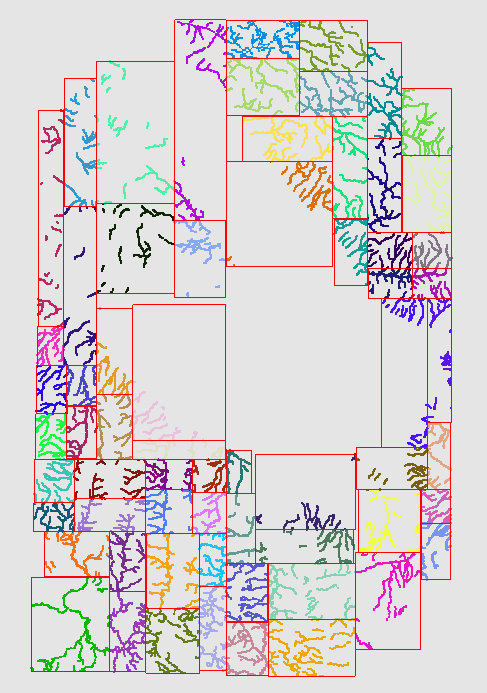
\includegraphics[scale=1.0]{ohbuchi.png}
  \caption{Разбиение карты на области}
  \label{pic_ohbuchi}
\end{figure}
Упомянутые выше спектральный анализ и внедрения водяных знаков производится для каждой области независимо.

Водяные знаки извлекаются сранением орининальной и атакованной карты. В первую очередь карты геометрически
''регистрируются'' с помощью итеративного процесса минимизации расстояния между множествами предварительно
выбранных пометок. Эта регистрация может устранить аффинное преобразование примененное к подписанной карте.

Для вставки вершин удаленных злоумышленником и удаления вершин вставленных злоумышленников используется 
следующий алгоритм. Для каждой вершины оригинальной
карты осуществляется поиск вершин в круге некоторого радиуса на атакованной карте. Если не было найдено ни одной,
вершины то соответсвующая вершина добавляется, если было найдено несколько, то удаляются все кроме ближайшей
к соответствующей вершине оригинальной карты.

Рассмотрим процесс внедрения ЦВЗ подробнее.  
Пусть $V = \{v_1, v_2, \dots, v_n\}$ есть множество вершин оригинальной карты, $n = |V|$. 
Пусть $\mathfrak{T}$ озбозначает некоторую триангуляцию множества $V$, $G(\mathfrak{T})$ обозначает 
граф триангуляции $\mathfrak{T}$. Собственные вектора $\{\mathbf{e}_i\}_{i=1}^n$ графа $G(\mathfrak{T})$ суть 
собственные вектора его лапласиана. 
Существует несколько определений лапласиана графа, к примему \cite{Biggs, Chung, Zhang}. В базовом алгоритме 
используется определение данное в \cite{Biggs}
$$R = I - D^{-1} A,$$ где $I$ --- единичная матрицв, $D$ --- диагональная матрица составленная из 
степеней вершин графа $G(\mathfrak{T})$, $A$ --- матрица смежности $G(\mathfrak{T})$
\begin{eqnarray*}
  D_{ij} = \begin{cases} deg(v_i) &\text{if $i = j$,} \\ 0 &\text{otherwise;} \end{cases} \\
  A_{ij} = \begin{cases} 1 &\text{if vertices $i$ and $j$ is adjacent,} \\ 0 &\text{otherwise.} \end{cases} 
\end{eqnarray*}
Собственные вектора $\{\mathbf{e}_i\}_{i=1}^n$ составляют базис $\mathbb{R}^n$. Будем предполагать, что 
собственные вектора нормализованны, $||e_i|| = 1$. 
Пусть $v_i = (x_i, y_i)$ тогда $\mathbf{r} = (r_1, r_2, \dots, r_n)$, $\mathbf{s} = (s_1, s_2, \dots, s_n)$ 
суть разложения векторов $\mathbf{x} = (x_1, x_2, \dots, x_n)^T$, $\mathbf{y} = (y_1, y_2, \dots, y_n)^T$ 
соответственно в базисе $\{\mathbf{e}_i\}_{i=1}^n$. Другими словами 
\begin{eqnarray*}
  \mathbf{x} = r_1 \mathbf{e}_1 + r_2 \mathbf{e}_2 + \dots + r_n \mathbf{e_n}; \\ 
  \mathbf{y} = s_1 \mathbf{e}_1 + s_2 \mathbf{e}_2 + \dots + s_n \mathbf{e_n}.  
\end{eqnarray*}
Если $\{\mathbf{e}_i\}_{i=1}^n$ ортогональны, то $r_i = (\mathbf{x}, \mathbf{e}_i)$, 
$s_i~=~(\mathbf{y}, \mathbf{e}_i)$, но в общем случае это не верно. 

Предположим, что внедряемое сообщение $\mathbf{m} = (m_1, m_2, \dots, m_k)$ состоит из $k$ бит, где $k \le n$, 
$m_i \in \{0, 1\}$. Введем обозначение $q_i = 2 * m_i - 1$, $q_i \in \{-1, 1\}$.
Изменим коэффициенты $r_i, s_i$, $1 \le k \le n$ следующим образом
\begin{eqnarray*}
  r_i' = r_i + \alpha p_i q_i; \\
  s_i' = s_i + \alpha p_i q_i, 
\end{eqnarray*}
где $\{p_i\}$ есть псевдослучайная последовательность, $\alpha$ --- некоторая положительная константа. 
Увеличение ~$\alpha$ увеличивает устойчивость к атакам на внедренные ЦВЗ, но вызывает большее искажение
карты. 

Пусть $\mathbf{x'}, \mathbf{y'}$ координаты вершин подписанной карты. 
\begin{eqnarray*}
  \mathbf{x'} - \mathbf{x} = (r_1' - r_1) \mathbf{e}_1 + (r_2' - r_2) \mathbf{e}_2 + \dots + (r_n' - r_n) \mathbf{e_n} = \\
  = \alpha \left[ p_1 q_1 \mathbf{e}_1 + p_2 q_2 \mathbf{e}_2 + \dots + p_k q_k \mathbf{e}_k \right], \\
  \mathbf{y'} - \mathbf{y} = \alpha \left[ p_1 q_1 \mathbf{e}_1 + p_2 q_2 \mathbf{e}_2 + \dots + p_k q_k \mathbf{e}_k \right]. 
\end{eqnarray*}
Другими словами внедрение ЦВЗ может быть выражено как построение вектора  
\begin{equation}
\label{formula:g}
 \mathbf{g} = \alpha \left[ p_1 \mathbf{h}_1 + p_2 \mathbf{h}_2 + \dots + p_k \mathbf{h}_k \right]; 
\end{equation}
$$ \mathbf{h_i} = \left( \begin{pmatrix} e_{i, 1} \\ e_{i, 1} \end{pmatrix} 
\begin{pmatrix} e_{i, 2} \\ e_{i, 2} \end{pmatrix}, \dots, \begin{pmatrix} e_{i, n} \\e_{i, n}  \end{pmatrix} 
\right), 1 \le i \le n. $$
Если вектора $\{\mathbf{e}_i\}_{i=1}^n$ ортонормированны, можно оценить среднее по всем вершинам расстояние 
смещения $\Delta v_{mean}$.
\begin{equation}
\label{formula:mean_displacement}
|\mathbf{g}| = \alpha * \sqrt {k} * \sqrt{2}; \mbox{      } \Delta v_{mean} = \alpha * \frac{\sqrt{2k}}{n}. 
\end{equation}

Для извлечение водяных знаков необходимо разложить вектора $\mathbf{x'} - \mathbf{x}$, 
$\mathbf{y'} - \mathbf{y}$ в базисе $\{\mathbf{e}_i\}_{i=1}^k$, то есть вычислить коэффициенты 
$\mathbf{u} = (u_1, u_2, \dots, u_k)$, $\mathbf{w} = (w_1, w_2, \dots, w_k)$, 
\begin{eqnarray*}
  \mathbf{x'} - \mathbf{x} = u_1 \mathbf{e}_1 + u_2 \mathbf{e}_2 + \dots + u_k \mathbf{e_k}; \\ 
  \mathbf{y'} - \mathbf{y} = w_1 \mathbf{e}_1 + w_2 \mathbf{e}_2 + \dots + w_k \mathbf{e_k}.  
\end{eqnarray*}
Биты внедренного сообщения получаются так:
$$q_i = \sgn(p_i * (u_i + w_i)), m_i = (q_i + 1) / 2.$$

\section{Обоснование корректности}
\label{sec:explanation}
Будем считать, что единственный вид атак, которым подвергается подписанная карта --- аддитивный случайный шум, примененный к координатам вершин, 
так как сопоставление множества вершин оригинальной и атакованной карты, применяемое в процедуре извлечения ЦВЗ базового алгоритма 
(\ref{sec:base}), позволяет свести все другие атаки также к добавлению к координатам вершин 
небольшой случайной (с точки зрения злоумышленника) величины.

Рассмотрим простейшую модель. Пусть действительное число $x$, чтобы закодировать бит $b = \pm 1$, преобразуется в $x' = x + b \alpha$, 
где $\alpha$~---~некоторая константа. Затем $x'$ атакуется случайным шумом c амплитудой $\sigma$, то есть преобразуется в $x'' = x' + y$,
где $y$ --- случайная величина с функцией распределения $F(t) = \Phi(t / \sigma)$, $\Phi$ --- функция Лапласа. Для извлечения бита вычисляется
$b' = \sgn(x'' - x)$. Вероятность того, что бит будет правильно извлечен, равна 
$
P[\sgn(x'' - x) = b] = P[\sgn(b \alpha + n) = b] = F(\alpha) = \Phi(\alpha / \sigma).
$

Чуть усложним модель. Пусть теперь для кодирования одного бита $b$ используется набор $\left\{x_j\right\}_{j=1}^n$
из $n=2k+1$ вещественных чисел, каждое из которых преобразуется также как в предыдущей модели,
для извлечения бита вычисляется $\sgn\left(\sum_{j=1}^n b_j'\right)$. Вероятность того, что бит будет извлечен правильно, равна 
$P\left(\left|\{j | b_j' = b, j = 1..n\}\right| \ge k + 1\right) = \sum_{j=0}^k \binom{n}{j} p^{n-j}(1-p)^j$, где $p = \Phi(\alpha / \sigma)$.
Если ввести обозначение $q = 1 - p$, $P_n = \sum_{j=0}^k \binom{n}{j} p^{n-j} q^j$, то будет верно следующее утверждение:
\begin{equation}
\label{prob_rec}
P_n = P_{n-2} + \binom{n-2}{k-1} p^k q^k (p - q),
\end{equation}
откуда видно, что для увеличения надежности кодирования бита можно увеличивать как $\alpha$, так и $n$. 
\begin{proof}
\begin{multline*}
\textstyle P_n = \binom{n}{0} p^{n} + \binom{n}{1} p^{n-1} q + \binom{n}{2} p^{n-2} q^2 + \ldots + \binom{n}{k-1} p^{k+2} q^{k-1} + \binom{n}{k} p^{k+1} q^k = \\
\shoveleft \textstyle = \left[\binom{n-1}{0} p^n + \binom{n-1}{0} p^{n-1} q \right] + \left[\binom{n-1}{1} p^{n-1} q + \binom{n-1}{1} p^{n-2} q^2 \right]
+ \ldots \\
\shoveright{\textstyle + \left[\binom{n-1}{k-1}p^{k+2}q^{k-1} + \binom{n-1}{k-1}p^{k+1}q^k \right] + \binom{n-1}{k}p^{k+1}q^k =} \\
\shoveleft \textstyle = \binom{n-1}{0} p^{n-1} + \binom{n-1}{1}p^{n-2}q + \ldots + \binom{n-1}{k-1}p^{k+1}q^{k-1} + \binom{n-1}{k} p^{k+1} q^k = \\
\shoveleft \textstyle = \left[\binom{n-2}{0}p^{n-1} + \binom{n-2}{0} p^{n-2} q \right] + \left[\binom{n-2}{0}p^{n-1} + \binom{n-2}{0} p^{n-2} q \right] +
\ldots \\
\shoveright{\textstyle + \left[\binom{n-2}{k-2}p^{k+2}q^{k-2} + \binom{n-2}{k-2}p^{k+1}q^{k-1} \right] + 
\binom{n-2}{k-1}p^{k+1}q^{k-1} + \binom{n-1}{k}p^{k+1}q^{k} = }\\
\shoveleft \textstyle = \left[\binom{n-2}{0} p^{n-2} + \binom{n-2}{1}p^{n-3}q + \ldots + \binom{n-2}{k-2}p^{k+1}q^{k-2} \right] + 
\binom{n-2}{k-1}p^{k+1}q^{k-1} + \binom{n-1}{k}p^{k+1}q^{k} = \\
\shoveleft \textstyle = P_{n-2} - \binom{n-2}{k-1}p^{k}q^{k-1} + \binom{n-2}{k-1}p^{k+1}q^{k-1} + \binom{n-1}{k}p^{k+1}q^{k} = \\ 
\shoveleft \textstyle = P_{n-2} + \binom{n-2}{k-1} p^{k}q^{k-1} (p - 1) + \left(\binom{n-2}{k-1} + \binom{n-2}{k} \right) p^{k+1}q^{k} = \\
\textstyle = P_{n-2} - \binom{n-2}{k-1} p^{k}q^{k} + 2p \binom{n-2}{k-1} p^k q^k = P_{n-2} + \binom{n-2}{k-1} p^k q^k (p - q). 
\end{multline*}
\end{proof}

Таким образом, для кодирования внедрения сообщения, состоящего из $m$ бит, можно было бы просто изменить координаты $m * n$ вершин карты на величину равную по модулю $\alpha$, где
$n$ и $\alpha$ выбираются из расчета того, какой амплитуды случайному шуму должны противостоять водяные знаки. Почему же все-таки выгоднее работать в частотной области?

Во-первых, длина внедряемого сообщения, как правило, много меньше числа вершин карты, а значит, чтобы изменение координат было равномерно 
по всем вершинам, надо выбирать достаточно большое $n$. В то же время из формулы~(\ref{prob_rec}) видно, что с ростом $n$ вероятность 
правильного извлечения сообщения растет довольно медленно, а значит с точки зрения устойчивости к атакам при одинаковом 
суммарном изменении координат вершин было бы выгодно брать небольшое значение $n$ и большое значение~$\alpha$.

Во-вторых, отметим, что переход от естественного базиса $\mathbb{R}^d$ к собственным векторам лапласиана, это есть в точности преобразование Фурье. 
А преобразование Фурье обладает принципом неопределенности, то есть, грубо говоря, невозможно произвольно сконцентрировать и функцию и ее Фурье-образ.
В частности для дискретного преобразования Фурье (ДПФ) в работе~\cite{Uncertainty} этот принцип сформулирован следующим образом. 
Пусть $\{\mathbf{j}\}_{j=0}^{d-1}$, $\{\tilde{\mathbf{k}}\}_{k=0}^{d-1}$ --- два ортонормированных базиса $\mathbb{C}^d$ связанных ДПФ:
\begin{equation*}
\textstyle |\tilde{\mathbf{k}} \rangle = \sum\limits_{j=0}^{d-1} \frac{e^{i 2\pi j k / d}}{\sqrt{d}} |\mathbf{j} \rangle,\mbox{    }
|{\mathbf{j}} \rangle = \sum\limits_{k=0}^{d-1} \frac{e^{i 2\pi j k / d}}{\sqrt{d}} |\tilde{\mathbf{k}} \rangle.
\end{equation*}
Если рассмотреть унитарные операторы 
$$
U = \sum\limits_{j=0}^{d-1} e^{i 2\pi j / d} |\mathbf{j} \rangle \langle \mathbf{j} |,\mbox{    }
U = \sum\limits_{k=0}^{d-1} e^{i 2\pi k / d} |\tilde{\mathbf{k}} \rangle \langle \tilde{\mathbf{k}} |,
$$
то их дисперсии
$$
\textstyle
\Delta U^2 = 1 - |\langle \psi | U | \psi \rangle |^2, \mbox{   }
\Delta V^2 = 1 - |\langle \psi | V | \psi \rangle |^2, \mbox{   } |\psi|^2 = 1,
$$
будут связаны соотношением $\Delta U^2 \Delta V^2 \ge \frac{\pi^2}{d^2}$ или $\Delta U^2 = (0|1), \Delta V^2 = (1|0)$. Отсюда в частности следует, что если вектор $\psi$ имеет координаты 
$\left(\frac{1}{\sqrt{d}}, \frac{1}{\sqrt{d}}, \ldots, \frac{1}{\sqrt{d}}\right)$ в одном базисе, он равен какому-то базисному вектору другого базиса.
В случае преобразования используемого в базовом алгоритме (и его модификации предложенной в данной работе) это тоже выполняется. Действительно, константный вектор на вершинах графа 
является его собственным вектором соответсвующим собственному числу $0$.

Считая, что вектор шума состоит из случайных величин с мат. ожиданием $0$ и одинаковой дисперсией, независимо заданных для каждой вершины графа, можно утверждать, 
что после преобразования Фурье они сконцентрируются около нескольких частот, а значит, большинство внедренных битов будет правильно извлечено с высокой вероятностью.


\section{Выводы к главе}
В данной главе была выполнена формальная постановка задачи, изложен базовый алгоритм и приведены не строгие рассуждения, обосновывающие его корректность.
